\section{Project Management \& Cost Estimation}

\subsection*{Project Timeline}
The development phase is designed to be lightweight and completed in approximately 6 weeks:

\begin{itemize}
    \item Requirement Analysis and Design: 0.5 week
    \item Backend Development (FastAPI): 1 week
    \item Frontend Development (Next.js): 1 week
    \item Database Setup (SQLite): 0.5 week
    \item Integration and Dockerization: 1 week
    \item Testing and Debugging: 1 week
    \item Deployment and Documentation: 1 week
\end{itemize}

\begin{figure}[htbp]
  \begin{center}
    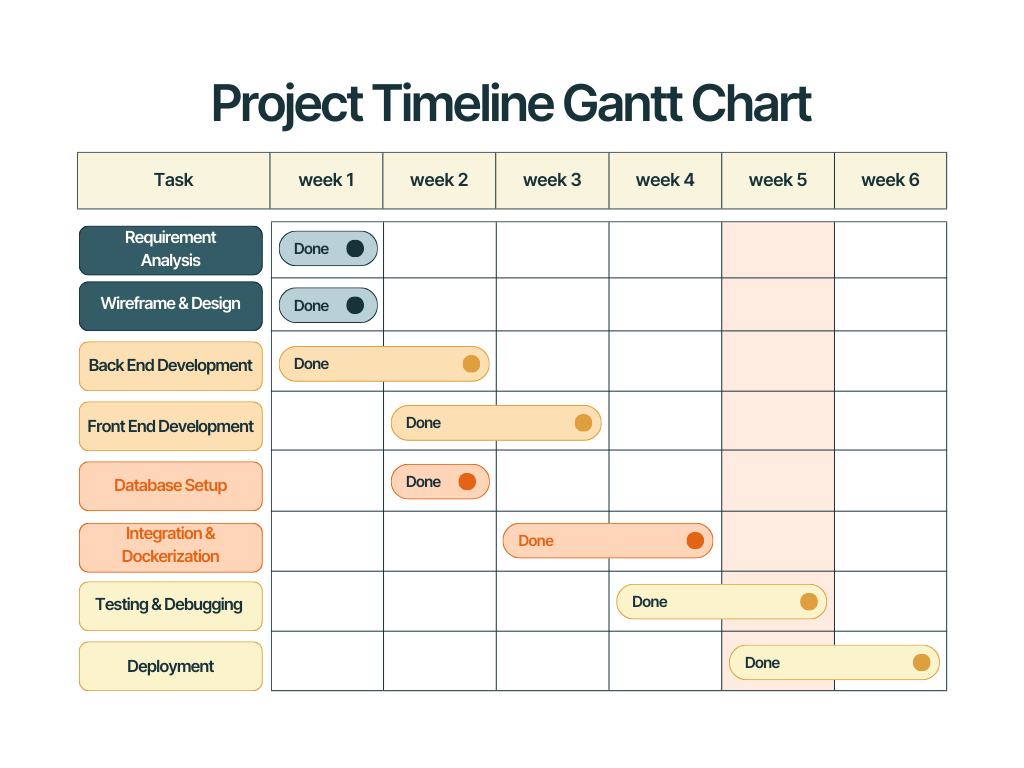
\includegraphics[width=0.85\textwidth]{figures/gantt-chart.png}
  \end{center}
  \caption{Gantt chart of project timeline.}\label{fig:gantt-chart}
\end{figure}


\subsection*{Cost Estimation}
The project is planned with minimal cost by leveraging free and open-source technologies:
\begin{itemize}
    \item \textbf{Development Effort:} The project is developed by a single developer
      as part of an academic exercise, so direct labor cost is negligible.
      If monetized, the equivalent effort can be valued at approximately \$500--\$800 (including the developer hiring cost).
    \item \textbf{Operational Costs:} VPS like Linode or AWS EC2 with minimal hardware configuration
      cost upto \$5-\$10 per month (for backend and database)  and
      Render (hosting) are sufficient for deployment.
      Docker is open-source and free. A custom domain is optional, costing about \$10 per year.
\end{itemize}

\noindent
\textbf{Overall Estimate:} The project can be developed with near-zero cost using free tiers,
with only optional expenses for a domain name.
